\section{Setup at Hj{\o}rring Library}
The initial steps of the setup was to determine the location at the library where the installation would be located. The library offered a series of different locations. The chosen location is in the middle of the library. The main reason for this choice was that the area had artificial lighting and the area is also the most direct path from the entrance to the working area and the children's area. In figure \ref{fig:library_floorplans} the layout of the library is shown along with the designated project area.

%During the last weeks of the project, the group setup the project at Hj{\o}rring Library in order to test it and make the final arrangements. The project itself requires a canvas, some illumination from infrared LEDs, an infrared camera and a projector.

Before the actual installation a model of the setup was created and discussed. The area selected provides a place for the projector since a broad sturdy row of shelves facing a the wall where the canvas will be deployed. Behind the canvas a strip of LEDs would be placed. Between the projector and the canvas there is a long display case, this will also be used to mount a strip of infrared LEDs. In figure \ref{fig:setup_model} the setup is illustrated:

\begin{figure}[htbp] 
\centering 
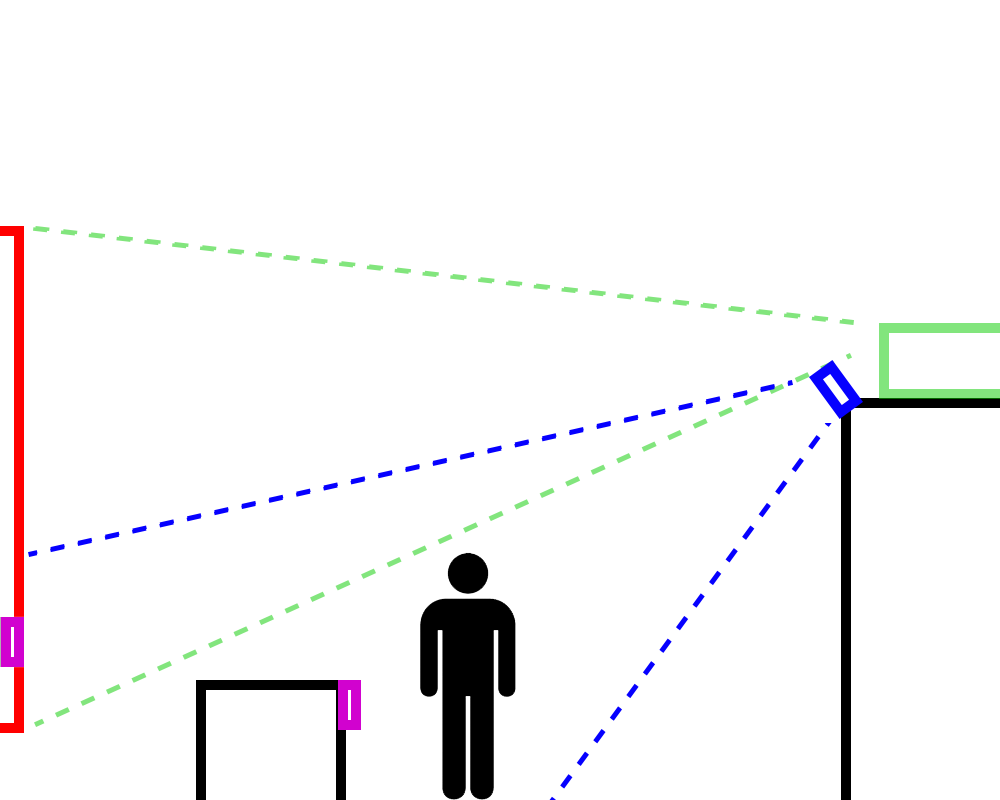
\includegraphics[width=0.8\textwidth]{Pictures/Setup/sideview_camera_with_person_two_strips.png} 
\caption{Model for the setup.} 
\label{fig:setup_model} 
\end{figure}

\begin{itemize}
\item Canvas is red
\item LED strip is purple
\item Camera with IR filter is blue, its field of view is outlined with blue.
\item The projector is faded green, its field of projection is outlined with faded green.
\end{itemize}

The feasibility of the model was tested during several visits at the library. The projectors and cameras placements were tested, and proved to be suitable for implementation. However there proved to be a problem with one of the two LED strips: The strip mounted on the wall did not, due to the angle of and distance to the camera, cover the intended ROI. Therefore adjustments were made to the installation, and one row of LEDs were removed. This maked the final installtion correspond to figure \ref{fig:setup_model_final}.

\begin{figure}[htbp] 
\centering 
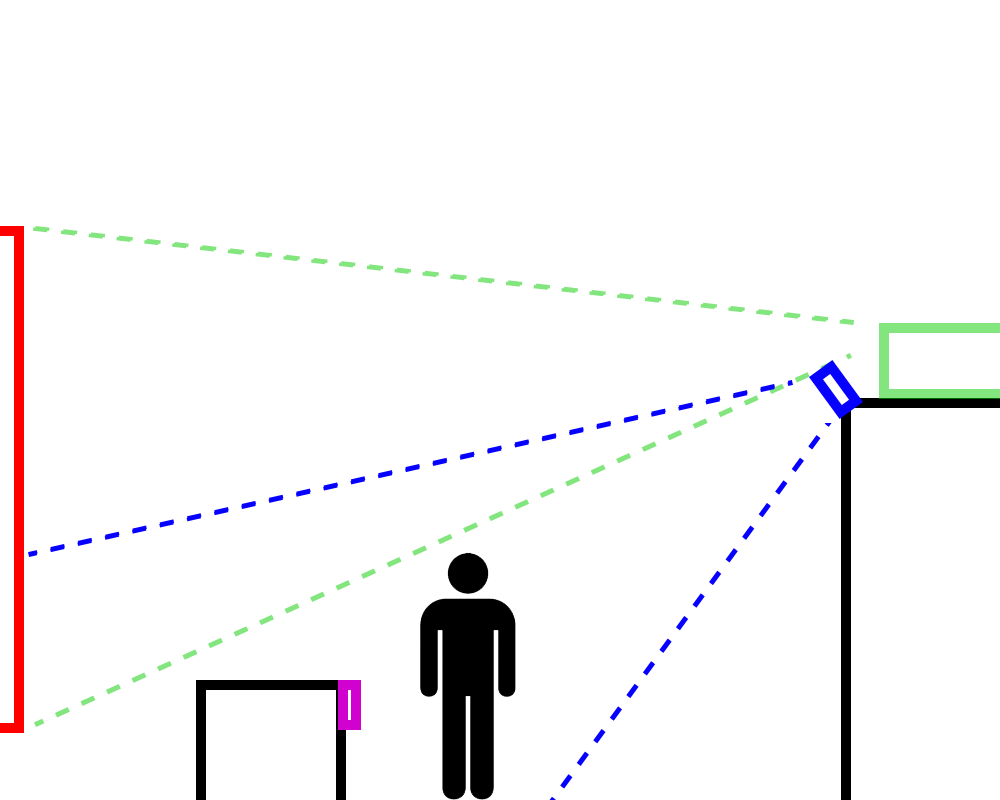
\includegraphics[width=0.8\textwidth]{Pictures/Setup/sideview_camera_with_person.png} 
\caption{The final setup as implemented at the library} 
\label{fig:setup_model_final} 
\end{figure}

The setup consists of different elements: Canvas, LED strips, power supply, computer and projector.

\begin{itemize}
\item LEDs strips

The first step on the construction of the Canvas was to position two LEDs strips in order to get the desired illumination for the infrared camera. As the placement of this project is a corridor divided by a red shelve that crosses the whole library, it was decided to add one strip on the lower part of this shelve and another LED stripes on the background covered by the canvas (see picture \ref{fig:LEDsPosition}).

\begin{figure}[htbp] 
\centering 
\includegraphics[width=0.8\textwidth]{Pictures/Design/stand1.png} 
\caption{Light as captured by a camera} 
\label{fig:LEDsPosition} 
\end{figure}

The construction of these LEDs stripes was made as simple as possible in order to lighten the weight. So finally the stripes were tapped to the shelves with duct tape. The solutions can be seen on Fig. \ref{fig:RealLEDs} and \ref{fig:RealRedLEDs}.

\begin{figure}[htbp] \centering
\begin{minipage}[b]{0.45\textwidth} \centering
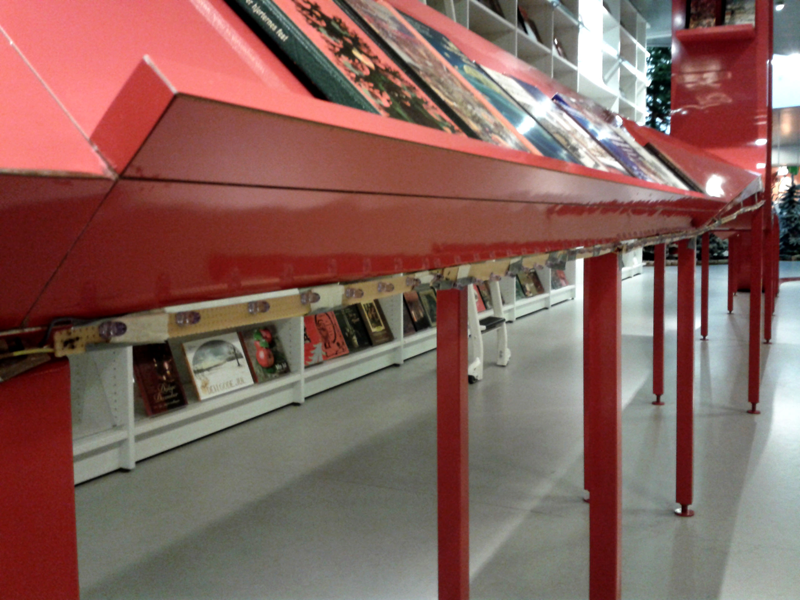
\includegraphics[width=1.00\textwidth]{Pictures/Design/LEDRedShelve.png}
\caption{LED stripes construction}
\label{fig:RealRedLEDs}
\end{minipage} \hfill
\begin{minipage}[b]{0.45\textwidth} \centering
\includegraphics[width=1.00\textwidth]{Pictures/Design/LEDShelve.png} 
\caption{LED stripes construction}
\label{fig:RealLEDs}
\end{minipage} \hfill
\end{figure}

\item Building the Canvas

For the projection it was decided to use a sheet to cover the 
\begin{figure}[htbp] 
\centering 
\includegraphics[width=0.8\textwidth]{Pictures/Design/stand2.png} 
\caption{Light as captured by a camera} 
\label{fig:CanvasPosition} 
\end{figure}

\end{itemize}

